
\chapter{OOP in Python}

\section{Introduction}

Classes in Python works in a similar way to classes in C++ seen before. However, Python classes are more flexible and powerful. In this chapter, we will see how to define classes in Python and how to use them.

\begin{codeblock}[language=Python]
class MyClass:
    def __init__(self, name):
        self.name = name

    def say_hello(self):
        print(f"Hello, {self.name}!")
\end{codeblock}

\begin{observationblock}[\plaintt{self}]
    Class methods have only one specific difference from ordinary functions: they must have an extra
    first name that has to be added to the beginning of the parameter list, but you do not give a value
    for this parameter when you call the method, Python will provide it. This particular variable refers
    to the object itself, and by convention, it is given the name \plaintt{self}.
\end{observationblock}

Also, the \texttt{\_\_init\_\_} method is run as soon as an object of a class is instantiated (i.e. created). The
method is useful to do any initialization (i.e. passing initial values to your object) you want to do
with your object. Notice the double underscores both at the beginning and at the end of the name.

We do not explicitly call the \texttt{\_\_init\_\_} method. It gets called when we create a new instance of the class.

Attributes can be instance-specific or shared among all instances. The first ones are defined outside the \texttt{\_\_init\_\_} method, while the second ones are defined inside the class but outside any method.

\begin{codeblock}[language=Python]
class Dog:
    kind = 'canine'         # class variable shared by all instances

    def __init__(self, name):
        self.name = name    # instance variable unique to each instance
\end{codeblock}

\begin{warningblock}
    Changing class attributes affect all instances!
\end{warningblock}

Besides regular methods, classes can have static methods and class methods. Static methods are methods that are not bound to an instance, while class methods are bound to the class itself.
\begin{itemize}
    \item \textbf{Static methods} are defined using the \texttt{@staticmethod} decorator.
    \begin{codeblock}[language=Python]
class MyClass:
    @staticmethod
    def static_method():
        print("This is a static method")
    \end{codeblock}
    \item \textbf{Class methods} are defined using the \texttt{@classmethod} decorator.
    \begin{codeblock}[language=Python]
class MyClass:
    @classmethod
    def class_method(cls):
        print("This is a class method")
    \end{codeblock}
    The \texttt{cls} parameter is the class itself.
\end{itemize}

\subsection*{Magic Methods}

Magic methods are special methods that have double underscores at the beginning and at the end of their names. They are also known as dunder methods. They allow us to emulate built-in behavior within Python and can be extremely useful when we want to implement operator overloading.

\begin{codeblock}[language=Python]
class MyClass:
    def __init__(self, name):
        self.name = name

    def __str__(self):
        return f"My name is {self.name}"
\end{codeblock}

\begin{observationblock}
    Notes for C++ programmers:
    \begin{itemize}
        \item The \texttt{self} in Python is equivalent to the \texttt{this} pointer in C++.
        \item All class members (including the data members) are public and all the methods are virtual in Python.
    \end{itemize}
\end{observationblock}


\section{Decorators}

Decorators in Python offer a powerful way to enhance the functionality of functions or methods.
They act as wrappers, allowing you to extend or modify the behavior of the original function.

Decorators can be imagined to be a shortcut to calling a wrapper function (i.e. a function that
"wraps" around another function so that it can do something before or after the inner function), so
applying the \texttt{@classmethod} is the same as calling 
\begin{codeblock}[language=Python]
    from_csv = classmethod(from_csv)
\end{codeblock}

\begin{definitionblock}
    Decorators are essentially functions that take another function as input, enhance its capabilities,
    and return a modified version of the original function.
\end{definitionblock}

\begin{codeblock}[language=Python]
def my_decorator(func):
    def wrapper():
        print("Something is happening before the function is called.")
        func()
        print("Something is happening after the function is called.")
    return wrapper

def say_hello():
    print("Hello!")

say_hello = my_decorator(say_hello)
\end{codeblock}

Or, with the \texttt{@} symbol:

\begin{codeblock}[language=Python]
@my_decorator
def say_hello():
    print("Hello!")
\end{codeblock}

This decorator, when applied to a function, surrounds the function call with additional actions.

It can be applied to classes as well:

\begin{codeblock}[language=Python]
def add_method(cls):
    def new_method(self):
        print("This is a new method")
    cls.new_method = new_method
    return cls

@add_method
class MyClass:
    def existing_method(self):
        print("This is an existing method")
    
obj = MyClass()
obj.new_method() # Prints "This is a new method"
\end{codeblock}

\begin{observationblock}
    Python comes with built-in decorators like \texttt{@staticmethod} and \texttt{@classmethod}, which are
    implemented in C for efficiency.
\end{observationblock}

Other than logging and timing/profiling, decorators can be used to add validation checks for
input parameters and output cleanup to functions or methods, or to implement caching
mechanisms, where the result of a function is stored for a specific set of inputs, and subsequent
calls with the same inputs can return the cached result.


\section{Inheritance and Polymorphism}

Inheritance in Python enables classes to inherit methods and attributes from other classes.
To use inheritance, we specify the base class names in a tuple following the class name in the
class definition. Next, we observe that the \texttt{\_\_init\_\_} method of the base class is explicitly called using the \texttt{self}
variable so that we can initialize the base class part of an instance in the subclass. This is very
important to remember.

\begin{warningblock}
    Python does not automatically call the constructor of the base class, you have to call it explicitly!
\end{warningblock}

In contrast, if we have not defined an \texttt{\_\_init\_\_} method in the subclass, the base class \texttt{\_\_init\_\_} method will be called automatically.

\begin{codeblock}[language=Python]
class Animal:
    def __init__(self, name):
        self.name = name

    def speak(self):
        raise NotImplementedError("Subclass must implement abstract method")

class Dog(Animal):
    def __init__(self, name):
        super().__init__(name)

    def speak(self):
        return f"{self.name} says Woof!"
\end{codeblock}

\subsection*{Getters}

Since attributes can change, one can use the \texttt{@property} decorator to define a getter method. This method is called when the attribute is accessed.

\begin{codeblock}[language=Python]
class Circle:
    def __init__(self, radius):
        self.radius = radius

    @property
    def diameter(self):
        return 2 * self.radius

    @property
    def area(self):
        return 3.14159 * self.radius ** 2
\end{codeblock}

\subsection*{Setters}

Similarly, one can use the \texttt{@<attribute>.setter} decorator to define a setter method. This method is called when the attribute is assigned a new value.

\begin{codeblock}[language=Python]
class Circle:
    def __init__(self, radius):
        self.radius = radius

    @property
    def diameter(self):
        return 2 * self.radius

    @diameter.setter
    def diameter(self, diameter):
        self.radius = diameter / 2
\end{codeblock}

This way we can ensure that the radius is always half the diameter.

\subsection*{Deleters}

Finally, one can use the \texttt{@<attribute>.deleter} decorator to define a deleter method. This method is called when the attribute is deleted.

\begin{codeblock}[language=Python]
class Circle:
    def __init__(self, radius):
        self.radius = radius

    @property
    def diameter(self):
        return 2 * self.radius

    @diameter.setter
    def diameter(self, diameter):
        self.radius = diameter / 2

    @diameter.deleter
    def diameter(self):
        del self.radius
\end{codeblock}


\section{Modules and Packages}

In Python, the ability to reuse code is facilitated by modules. A module is a file with a \texttt{.py}
extension that contains functions and variables. There are various methods to write modules,
including using languages like C to create compiled modules.
When importing a module, to enhance import performance, Python creates byte-compiled files
\texttt{(\_\_pycache\_\_/filename.pyc)}. These files, platform-independent and located in the same
directory as the corresponding \texttt{.py} files, speed up subsequent imports by storing preprocessed
code.

You can import modules in your program to leverage their functionality. For instance, consider the
\texttt{sys} module in the Python standard library. Below is an example:
\begin{codeblock}[language=Python]
import sys

print("Command line arguments: ", sys.argv)
\end{codeblock}

You can selectively import variables from a module using the \texttt{from... import...} statement.
However, it's generally advised to use the \texttt{import} statement to avoid potential name clashes and
enhance readability.

\begin{codeblock}[language=Python]
    from math import pi
    print("The value of pi is", pi)
\end{codeblock}

\begin{observationblock}
    Every module has a \plaintt{\_\_name\_\_} attribute that defines the name of the module. When the
    interpreter reads a source file, it sets the \plaintt{\_\_name\_\_} variable to \plaintt{"\_\_main\_\_"} if the
    module is being run as the main program. Otherwise, it sets the variable to the module's name.
\end{observationblock}

You can create your own modules by writing a Python file and importing it in another file. To
import a module, you can use the \texttt{import} statement followed by the module name. You can also
import specific functions or variables from a module using the \texttt{from... import...} statement.

Moreover, the \texttt{dif()} function lists all symbols defined in an object. For a module, it includes
functions, classes, and variables. It can also be used without arguments to list names in the
current module.

\section{Packages}

Packages are folders of modules with a special \texttt{\_\_init\_\_.py} file, indicating that the folder
contains Python modules. They provide a hierarchical organization for modules.

\begin{figure}
    \centering
    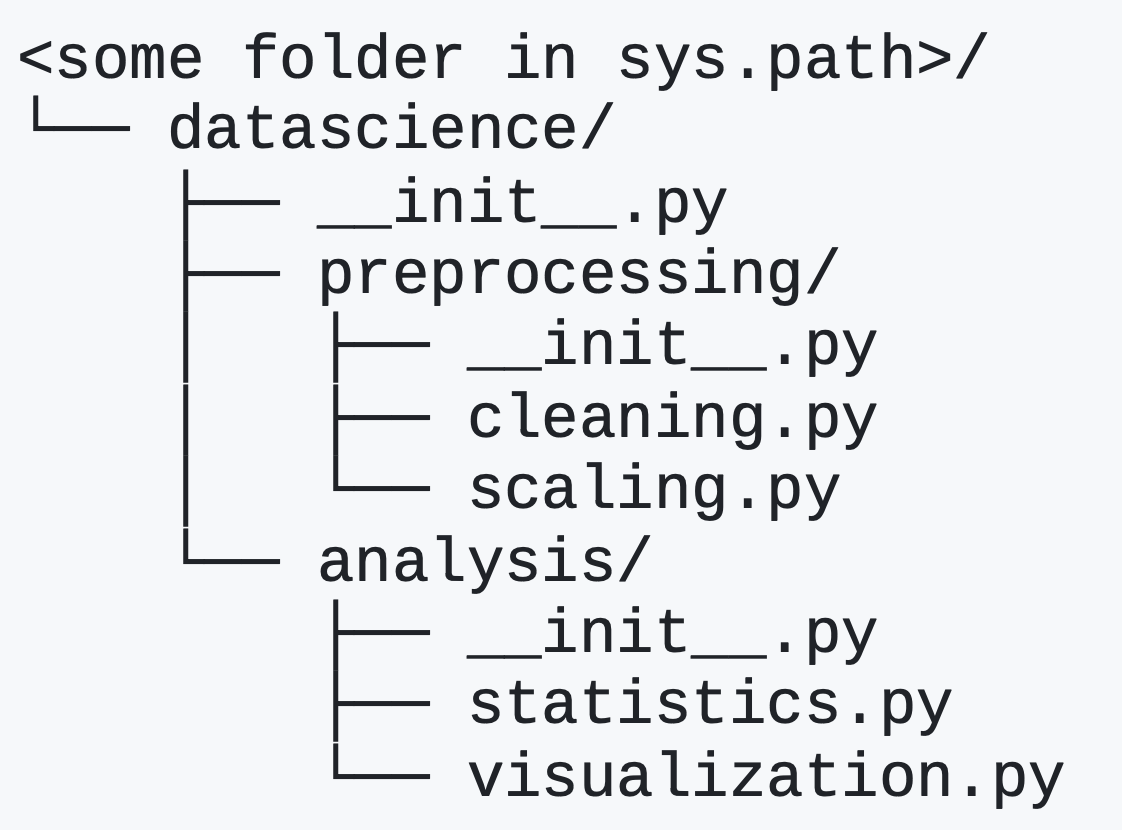
\includegraphics[width=0.5\textwidth]{assets/py_packages.png}
    \caption{Package Structure}
    \label{fig:packages}
\end{figure}

\begin{observationblock}
    The \plaintt{\_\_init\_\_.py} file in a Python package serves multiple purposes. It's executed when the
    package or module is imported, and it can contain initialization code, set package-level variables,
    or define what should be accessible when the package is imported using \plaintt{from package import *}.
\end{observationblock}
